
\documentclass[10pt,twocolumn,letterpaper]{article}

\usepackage{iccv}
\usepackage{times}
\usepackage{epsfig}
\usepackage{graphicx}
\usepackage{amsmath}
\usepackage{amssymb}
\usepackage[numbers,sort]{natbib}
\usepackage[UTF8]{ctex}


\usepackage{subfigure}
\usepackage{upgreek}
\usepackage{multirow}
\usepackage{color}
\usepackage{bm}
\DeclareMathOperator*{\argmin}{arg\,min}
\usepackage{arydshln}
\usepackage{latexsym}

\usepackage{amsthm}
\newtheorem{theorem}{Theorem}
\newtheorem{lemma}[theorem]{Lemma}
\newtheorem{conj}[theorem]{Conjecture}

% Include other packages here, before hyperref.

% If you comment hyperref and then uncomment it, you should delete
% egpaper.aux before re-running latex.  (Or just hit 'q' on the first latex
% run, let it finish, and you should be clear).
\usepackage[pagebackref=true,breaklinks=true,letterpaper=true,colorlinks,bookmarks=false]{hyperref}

% \iccvfinalcopy % *** Uncomment this line for the final submission

\def\iccvPaperID{1} % *** Enter the ICCV Paper ID here
\def\httilde{\mbox{\tt\raisebox{-.5ex}{\symbol{126}}}}

% Pages are numbered in submission mode, and unnumbered in camera-ready
\ificcvfinal\pagestyle{empty}\fi
\begin{document}

%%%%%%%%% TITLE
\title{A Benchmark Dataset for Evaluating Denoising and Demosaicking Algorithms}

\author{First Author\\
Institution1\\
Institution1 address\\
{\tt\small firstauthor@i1.org}
% For a paper whose authors are all at the same institution,
% omit the following lines up until the closing ``}''.
% Additional authors and addresses can be added with ``\and'',
% just like the second author.
% To save space, use either the email address or home page, not both
\and
Second Author\\
Institution2\\
First line of institution2 address\\
{\tt\small secondauthor@i2.org}
}

\maketitle
%\thispagestyle{empty}


%%%%%%%%% ABSTRACT
\begin{abstract}
In this paper, we propose to simultaneously employing the spatial and temporal information to construct a real-world dataset which contain the original raw images as well as corresponding ``ground truth'' images. This dataset can be used in real world image denoising, demosaicking, and joint denoising and demosaicking (JDD) problems.
\end{abstract}

%%%%%%%%% BODY TEXT
\section{Introduction}

According to \cite{healey1994radiometric}, the noise corrupted in the imaging process is signal dependent and comes from five main sources:\ photon shot, fixed pattern, dark current, readout, and quantization noise.

Recently, Nam et al. constructed a realistic noisy images dataset \cite{crosschannel2016}, which includes noisy images of 11 static scenes.\ The noisy images were collected under controlled indoor environment.\ Each scene was shot 500 times under the same camera and camera setting.\ The mean image of the 500 shots is roughly taken as the ``ground truth'', with which the PSNR can be computed. Since the image size is very large (about $7000\times5000$) and the 11 scenes share repetitive contents, the authors of \cite{crosschannel2016} cropped 15 smaller images (of size $512\times512$) to perform experiments.\

Although this dataset has been used for analysis of real image noise, there are several problems on this dataset. The major problems are summarized as follows:

\textbf{Problem 1}: These 500 images for each scene are averaged on sRGB space, which is not reasonable. Only on the raw images, the realistic noise is independent with the noise on other pixels of the camera sensor. After the in-camera imaging processing pipeline \cite{NewInCamera,crosschannel2016,karaimer_brown_ECCV_2016}, the noise is no longer independent at all. Besides, the dark current generated by heat follows Poisson distribution, while the noise generated during the readout process follows Gaussian distribution. But only on the raw images, the realistic noise can be modeled as mixed Poisson and Gaussian distribution. After the above mentioned pipeline, the noise would be much more complex and cannot be modeled by simple mixed Poisson and Gaussian distribution.

\textbf{Problem 2}: 连续拍摄500张图持续时间必然很长,对周围环境要求过高。因此这个方法只能用于拍摄固定光源下的,室内的,静态的物体。无法拍摄人像,自然光下的物体,在短时间内静止但是在长时间内可能有轻微运动的物体。举个例子,Nikon A7II相机1秒钟只能连续拍摄60张图片,拍摄500张图片需要9分钟左右,即便是在室内,如果有自然光招进来,那么自然光的变化会严重影响拍摄的光照条件。在室外拍摄的时候,连续拍摄9分钟更加不可能拍摄到内容和光照一致的连续500张图片。

主要问题3:连续拍摄500张图像,raw data的像素有很大可能存在位移(shift),从而导致Color Filter Array (CFA)图片的R, G, B通道上的数值产生位移,从而导致demosaicking的时候产生偏差。 另外,还会使得图片的edge部分产生zippering的瑕疵、texture部分产生轻微模糊等问题。

主要问题4:连续拍摄500张会使得相机的传感器因为连续工作产生大量的热,从而使得相机在后续拍摄中产生大量的电子,温度越高,噪声越大,就是如下相机噪声模型中的$\bm{D}$的均值和方差越大。
\begin{equation}
\bm{P} = f((g_{cv}(\bm{C}+\bm{D})+\bm{N}_{reset})g_{out}+\bm{N}_{out})+\bm{Q}
\end{equation}

主要问题5:连续拍摄500张图取平均,那么传感器的每个pixel产生的噪声还带有该pixel本身的属性,这个由于物理性质本身产生的噪声无论如何也无法通过平均去掉,比如某个pixel总是把测量到的数值变大,这个测量值与真实值之间的差异无法通过自身上的平均消除。如果再借用空间上的信息,那么这个pixel产生的总是偏大噪声可以被周围pixel的测量值拉回到平均位置。


主要问题6:对于某些特定的相机,比如DJI的无人机Phonton 3,其只能一次性连续拍摄10张左右的照片。在下一次连续拍摄的时候,相机会自动进行聚焦等操作,而我们无法保证这些相机在相邻两次连续拍摄之间拥有完全一样的参数。只能把这一次性拍得的10张图片视为参数一致的图片数据,与之后连续拍摄的图片之间取平均会使得图片产生非常明显的位移和模糊。


解决办法:对于问题1,我们应该在raw data上取平均,而不是在RGB空间里取平均。对于问题2,3,4,5,我们可以用每张图片的空间信息来换取时间上的信息。我们不需要连续拍摄500张图片,也许只需要拍摄10张左右的图片,再利用空间上的信息就可以得到``ground truth''的图片了。如何利用空间上的信息呢?那就是在CFA上的RGGB像素里取平均,这个想法来自于微软公司的研究人员在CFA上做demosaicking数据库的构造\cite{khashabi2014joint}。这也是我们接下来要介绍的只在CFA空间域里取平均构建``ground truth''的工作。


Khashabi et al.在发表于TIP2014的文章\cite{khashabi2014joint}里构造了一个数据量很大的demosaicking的数据库,作者对于每个场景都做下采样。在下采样的过程中,把大小为$W\times W$的块中的代表某个颜色(比如红色)的所有像素取平均,然后下采样成一个像素;在右侧相邻的$W\times W$块中对另一个颜色(比如绿色)的所有像素取平均,然后下采样成一个像素;在下方响铃的$W\times W$块中对一个颜色(比如绿色)的所有像素取平均,然后下采样成一个像素;在右下方响铃的$W\times W$块中对另一个颜色(比如蓝色)的所有像素取平均,然后下采样成一个像素。这样就可以把一个$2W\times2W$的CFA中的块下采样成一个大小为$2\times2$的块,而且是符合``RGGB''的采样pattern(对其他采样pattern也可以用类似的方法)。这个下采样模式可以通过图1表示。

\begin{figure}
\centering
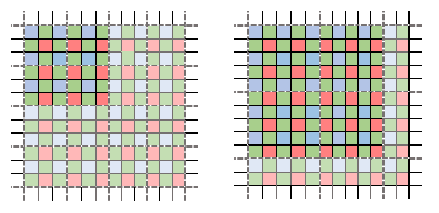
\includegraphics[width=0.95\linewidth]{CFA.png}
\caption{Averaging with odd windows, with $W = 1$ (left) and $W = 2$ (right),
where the window size is $(2W + 1)\times (2W + 1)$.
}
\label{fig1}
\end{figure}


主要问题1:存在图片像素过小,每张图片只有$200\times200$的大小。这是因为,为了得到干净的CFA图片,需要采用很大的下采样倍数。比如原图可能有$4000\times4000$,但是为了得到干净的CFA图片,采用$20\times20=400$倍的下采样倍数,才能得到一张非常干净的CFA图片可以用于做真实的demosaicking实验。这极大地降低了图片的内容和多样性,失去了图片原有的文理信息。这种失真严重的结果就是,在这个数据集上训练得到的demosaicking的算法不鲁棒,很容易遇到这个训练集上没有的图像块结构和文理信息。这时候我们可以借用时间上的信息,比如同样的图片拍摄10张,这10张的拍摄在0.1秒左右,在可控制的情况下,图片内容是可以保持不变的。在这种情况下,也许在空间上,我们不需要下采样那么多倍数,可以只下采样$4\times4=16$倍左右,那么依然可以得到$1000\times1000$大小的图片,依然可以保留大部分的文理,同时还可以得到质量一样的``ground truth''。

综上所述,我们可以结合时间上的多次采样和空间上的下采样,得到可以同时用于真实去噪和真实demosaicking的数据库。这个数据库还有用于真实的超分辨算法训练的潜在的可能性。



{
\small
\bibliographystyle{unsrt}
\bibliography{egbib}
}

\end{document}
